\documentclass[a4paper,11pt]{article}
\usepackage[T1]{fontenc}
\usepackage[utf8]{inputenc}
\usepackage[francais]{babel}
\usepackage[top=3cm, bottom=3cm, left=3cm, right=3cm]{geometry}
\usepackage{lmodern}

% Pour avoir de belles url
\usepackage{url}
\urlstyle{sf}
% Pour utiliser des images
\usepackage{graphicx} 
\graphicspath{{img/}}
% Pour utiliser l'index
\usepackage{makeidx}
\makeindex

% couleurs
\usepackage{color}
\definecolor{bleuClair}{rgb}{0,0.4,0.9}
\definecolor{bleuFonce}{rgb}{0,0.3,0.6}
\definecolor{grisFonce}{gray}{0.25}

% Pour mettre du code source
\usepackage{listings}
\lstnewenvironment{PHP}{
  \lstset{
    frame=trBL,
    language=PHP,
    basicstyle=\ttfamily,
    keywordstyle=\color[rgb]{0,0,1},
    commentstyle=\color[rgb]{0.133,0.545,0.133},
    stringstyle=\color[rgb]{0.627,0.126,0.941},
    showspaces=false,
    showstringspaces=false,
    morekeywords={class, extends, public, function},
    breaklines=true,
  }
}{}
\lstnewenvironment{HTML}{
  \lstset{
    frame=trBL,
    language=HTML,
    basicstyle=\ttfamily,
    keywordstyle=\color[rgb]{0,0,1},
    commentstyle=\color[rgb]{0.133,0.545,0.133},
    stringstyle=\color[rgb]{0.627,0.126,0.941},
    showspaces=false,
    showstringspaces=false,
    breaklines=true,
  }
}{}

\title{MINZ Is Not Zend\\{\small version 1.0}\\\textbf{Documentation\\ {\small en cours de rédaction}}}
\author{Marien Fressinaud}

\makeatletter
\renewcommand\section{\@startsection{section}{1}{\z@}%
	{2cm \@plus -1ex \@minus -.2ex}%
	{2.3ex \@plus.2ex}%
	{\color{bleuClair}\reset@font\Large\bfseries}}

\renewcommand{\subsection}{\@startsection{subsection}{2}{\z@}%
             {-3.25ex\@plus -1ex \@minus -.2ex}%
             {1.5ex \@plus .2ex}%
             {\color{bleuFonce}\normalfont\large\bfseries}}
\makeatother

\begin{document}

\maketitle

%%%%%%%%%%%%%%%%%%%%%%%%%%%%%%%%%%%%%%%%%%%%%%%%%%%%%%%%%%%%%%%
\newpage
\tableofcontents
\newpage
%%%%%%%%%%%%%%%%%%%%%%%%%%%%%%%%%%%%%%%%%%%%%%%%%%%%%%%%%%%%%%%
\section{Fonctionnement général}
\subsection{Principes fondamentaux}
Pour bien commencer cette documentation, il est important de définir ce qu'est MINZ et de délimiter l'usage qu'il est possible d'en faire.\\

MINZ est un \textbf{framework PHP}, c'est-à-dire qu'il propose une architecture particulière pour l'écriture d'application PHP. On peut le voir comme un squelette, et l'application comme les muscles, cerveaux, peau, etc. Ce framework repose lui-même sur la \textbf{modélisation MVC} (pour Model View Controller). Le modèle MVC permet de séparer logiquement les données (un utilisateur avec un nom, un prénom, un mot de passe par exemple), leur représentation (la façon dont on va les afficher) et leur traitement. Cela permet d'avoir une application facile à maintenir.\\

MINZ est fortement inspiré de \textit{Zend Framework}, qui est un autre framework PHP. Bien qu'inspiré, il s'en éloigne par bien des aspects, d'où son nom en clin d'oeil : \textit{MINZ Is Not Zend}. Il se veut notamment bien plus léger et plus facile à mettre en place afin de faciliter le déploiement d'applications MINZ. Si vous connaissez déjà Zend Framework, il est certain que vous y trouverez de nombreuses similitudes, notamment au niveau de l'architecture.\\

J'ai dans l'idée de rendre MINZ ``compatible'' XMPP. C'est-à-dire que la création d'applications reposant sur XMPP sera grandement facilité. Cela pour démocratiser ce protocole très puissant, et surtout très utile.\\

Si vous souhaitez démarrer rapidement dans le domaine des frameworks, je ne peux que vous conseiller de commencer par MINZ ! :)

\subsection{Architecture}
MINZ repose sur trois répertoires principaux :
\begin{itemize}
  \item \texttt{app} : C'est dans celui-ci que tout le code PHP/HTML de l'application sera écrit, vous n'aurez donc à vous préoccuper \textbf{presque} que de celui-ci.
  \item \texttt{lib} : Tout le code du framework en lui-même se trouve ici, en principe vous n'avez pas besoin d'y toucher. Nous verrons plus tard qu'il est possible d'écrire sa propre librairie, qui se retrouvera donc ici.
  \item \texttt{public} : C'est la partie accessible de l'extérieur, on y retrouve le fichier \texttt{index.php} principal qui lance l'application ainsi que les thèmes, les scripts javascript, les images, etc. Nous verrons plus loin qu'il est possible de mettre son contenu à la racine si jamais on ne peut pas faire pointer le nom de domaine sur ce répertoire.
\end{itemize}

Comme dit ci-dessus, le répertoire \texttt{app} est le plus important car c'est celui-ci qui contiendra les contrôleurs, modèles et vues ainsi que d'autres éléments que nous détaillerons plus loin.\\

Un schéma du fonctionnement est sans doute nécessaire pour bien comprendre comment tout cela fonctionne :
\begin{figure}[h]
  \centering
  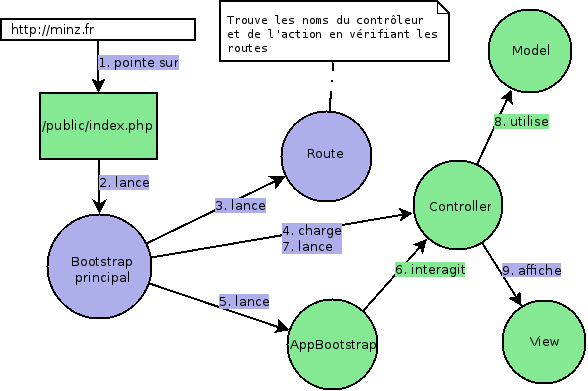
\includegraphics[width=13cm]{schemaFonctionnement.png}
  \caption{Schéma du fonctionnement de MINZ}
  \label{fig1}
\end{figure}

Ce qu'il faut voir ici, c'est l'enchaînement des actions (représentées par les flèches) et comprendre les couleurs. Les ronds représentent des classes PHP. On pourra noter des soucis d'enchaînement (je pense surtout au lancement de la classe Route). Cela devrait être revu dans la version 2 de MINZ, grâce notamment à l'utilisation des \textit{design patterns}.

Les flèches sont numérotées de 1 à 9, et c'est donc l'ordre dans lequel se déroule le fonctionnement du framework. On peut donc voir que lorsque l'url \url{http://minz.fr} est demandée, on va d'abord chercher le fichier \texttt{/public/index.php} qui se charge de lancer le \texttt{Bootstrap}, qui va lui-même demander à récupérer le nom du contrôleur et de l'action à la classe \texttt{Route}, etc.

Pour ce qui est des couleurs, tout ce qui est en bleu représente des classes et méthodes dont vous n'avez pas à vous soucier puisque c'est le framework qui s'en charge lui-même. Tout ce qui est de couleur verte, c'est à vous de le coder. Notez toutefois, si on prend l'exemple du contrôleur, que celui-ci hérite d'une classe parente, donc vous n'avez pas \textbf{tout} à écrire. Si vous avez suivi, en principe, le bleu se trouve dans le répertoire \texttt{lib}, et le vert, dans le répertoire \texttt{app} (à l'exception de \texttt{index.php} qui se trouve dans \texttt{public}).\\

Si tout cela vous paraît un peu obscur, c'est sans doute que mon schéma est mauvais... ou que l'architecture n'est pas terrible... ou les deux ! Il ne tient qu'à vous de me le faire savoir.\\

Par ailleurs, il est important de bien comprendre l'importance de l'action et du contrôleur qui lui est associé. Le framework nécessite de ces deux informations pour fonctionner. Pour cela, on lui indique via l'URL avec la variable \texttt{\$\_GET['c']} le nom du contrôleur à exécuter. La variable \texttt{\$\_GET['a']} sert à donner le nom de l'action. Concrètement, le contrôleur sert à indiquer ce que l'on veut manipuler (par exemple, un Utilisateur) et l'action, une opération à faire sur ce contrôleur (par exemple, ajouter un Utilisateur en base de données).

\subsection{Pré-requis et installation}
Comme il est indiqué dans le fichier \texttt{README} fourni avec le framework, MINZ ne requiert que de peu de choses. La première est \textbf{un serveur Apache} pour l'hébergement. Il a besoin aussi de \textbf{PHP 5}. Pour le moment, je sais qu'il fonctionne sur PHP 5.2.9 et supérieur, mais je pense que des versions antérieures devraient fonctionner aussi. MINZ n'utilise pas beaucoup de fonctions ``exotiques''. Enfin, activer l'\textbf{URL Rewriting} est recommandé pour pouvoir utiliser correctement le système de routes. Sachez toutefois qu'il n'est pas obligatoire (vous devrez utiliser alors des URLs plus traditionnelles). Tout ceci est expliqué plus loin.\\
Et c'est tout ce que je préconise pour pouvoir utiliser le framework, soit des choses que l'on trouve chez la plupart des hébergeurs.\\

Passons à l'installation. Là encore, c'est assez simple. Pour le moment, vous pouvez trouver le code complet sur la page GitHub dédiée :\\ \url{https://github.com/marienfressinaud/MINZ}\\

Une fois les sources téléchargées, il ne vous reste plus qu'à décompresser l'archive sur votre serveur. Assurez-vous que votre nom de domaine pointe sur le répertoire \texttt{public} et modifiez le nom de domaine dans le fichier de configuration (\texttt{/app/configuration/application.ini}). Rendez-vous sur votre site à partir de votre navigateur, et vous devriez voir apparaître l'application par défaut de MINZ ! Félicitations.\\

\textbf{Remarque} : \textcolor{grisFonce}{il se peut que vous ne puissiez faire pointer votre nom de domaine au bon endroit. Deux solutions s'offrent à vous :
\begin{enumerate}
  \item Coupez/collez le contenu de \texttt{public} dans le répertoire dans lequel pointe votre nom de domaine. Des modifications sont alors à porter aux constantes de chemins dans le contenu de \texttt{index.php}.
  \item Dans le fichier de configuration, lors de la modification du nom de domaine, ajoutez le chemin complémentaire. Par exemple, vous aurez la ligne \texttt{domain = "http://www.minz.test/public"} si votre nom de domaine pointe sur le répertoire parent de \texttt{public}.
\end{enumerate}
}

\newpage
%%%%%%%%%%%%%%%%%%%%%%%%%%%%%%%%%%%%%%%%%%%%%%%%%%%%%%%%%%%%%%%

\section{Développer avec MINZ}
\subsection{Bien commencer : comprendre le index.php}
Le code de ce fichier est déjà écrit par défaut dans le framework fourni. Il est toutefois important de le comprendre car c'est par là que tout commence. Le code que l'on peut trouver est (à quelque chose près) le suivant :
\begin{PHP}
<?php
// Constantes de chemins
define('PUBLIC_PATH', realpath(dirname(__FILE__)));
define('LIB_PATH', realpath(PUBLIC_PATH.'/../lib'));
define('APP_PATH', realpath(PUBLIC_PATH.'/../app'));
define('LOG_PATH', realpath(PUBLIC_PATH.'/../log'));
define('CACHE_PATH', realpath(PUBLIC_PATH.'/../cache'));

// Ajout du repertoire /lib dans l'include_path
set_include_path(get_include_path().PATH_SEPARATOR.LIB_PATH);

// Parametres du lancement de l'application
$params = array(
'config_file' => APP_PATH.'/configuration/application.ini'
);

require_once('Bootstrap.class.php');

$bootstrap = Bootstrap::getInstance($params);
$bootstrap->init(); // lancement de l'application
\end{PHP}

Le principe ici est d'abord de définir des constantes pour les différents chemins pour faciliter leur utilisation. Ensuite, nous ajoutons notre chemin de librairie à l'\texttt{include\_path} afin de pouvoir inclure les fichiers de librairie en indiquant simplement leur nom plutôt que leur chemin complet.\\

Le chemin vers le fichier de configuration est défini dans un tableau de paramètres. On pourra imaginer dans le futur ajouter d'autres informations à ce tableau.\\

Enfin, on lance le \texttt{Bootstrap}. Tout cela est plutôt simple et ne devrait pas poser de problème mais je pense qu'il est important d'en parler, ne serait-ce que pour avoir connaissance des constantes de chemins qui sont très utiles.

\subsection{Tour d'horizon du répertoire application}
Le répertoire \texttt{app} regroupe à peu près tous les fichiers que vous aurez à écrire. Son contenu est principalement du PHP, mais contient aussi du HTML pour les vues (l'extension est en fait .phtml pour pouvoir utiliser un peu de PHP à l'intérieur quand même). On y retrouve
\begin{itemize}
  \item le répertoire \texttt{configuration} qui contient le fichier de configuration mais aussi le fichier décrivant les routes (nous y reviendrons après)
  \item le répertoire \texttt{controllers} regroupe les contrôleurs de l'application
  \item le répertoire \texttt{models} regroupe les modèles de l'application (y compris ceux permettant d'accéder à la base de données, et autres systèmes de persistance)
  \item le répertoire \texttt{views} regroupe les vues de l'application. À l'intérieur, les vues sont regroupées par contrôleurs et nommées selon l'action qu'elle représente. Ainsi, la vue associée à l'action \texttt{login} du contrôleur \texttt{utilisateur} est representée sur le système de fichier par\\\texttt{/app/views/utilisateur/login.phtml}.
  \item le répertoire \texttt{layout} contient le squelette HTML du site.
  \item le fichier \texttt{AppBootstrap.php} est le Bootstrap de l'application lui permettant d'automatiser un certain nombre d'actions à son lancement.
\end{itemize}

\subsection{Écrire un Controller}
Tout d'abord, la norme pour les fichiers de contrôleurs veut que ceux-ci se trouvent dans le répertoire \texttt{/app/controllers} et que leur nom soit de la forme \texttt{nomController} (où \texttt{Controller} est commun à tout contrôleur). Attention à ce que la casse (majuscule/minuscule) corresponde entre le nom de fichier, le paramètre \texttt{\$\_GET['c']} de l'URL et le nom de classe.\\

Le code minimal d'un contrôleur est très simple :
\begin{PHP}
<?php   
class indexController extends Controller {
  public function indexAction() {}
}
\end{PHP}

Il y a deux trois choses à noter ici.\\

Le nom de la classe est ici le nom que l'on passera par l'URL (à l'aide de la variable \texttt{\$\_GET['c'])}.\\

De plus, notre contrôleur hérite de la classe \texttt{Controller}. Cela induit quelques petits éléments, notamment l'accès à la \texttt{View} à travers l'attribut \texttt{\$this->view}. Nous verrons dans la partie suivante les actions que l'on peut lui appliquer. Ensuite, les méthodes \texttt{firstAction()} et \texttt{lastAction()} peuvent être redéfinies. Ce sont des actions qui vont se lancer avant et après chacune des actions que vous allez écrire par la suite pour ce contrôleur particulier.\\

Enfin la méthode \texttt{indexAction} correspond à l'action \texttt{index} (l'action par défaut pour tout contrôleur). Vous aurez donc à écrire d'autres actions. Celles-ci se lanceront en fonction du paramètre \texttt{\$\_GET['a']} passé dans l'URL. Vous pourrez manipuler la vue à l'intérieur de ces méthodes. Par exemple, si votre méthode correspond à l'accueil de votre site, vous pouvez ajouter un titre comme ceci :
\begin{PHP}
public function indexAction() {
  $this->view->appendTitle('Accueil - ');
  // ou
  $this->view->prependTitle(' - Accueil');
}
\end{PHP}

La syntaxe sera expliquée plus loin mais est tout de même simple à comprendre.\\

Ainsi, dans ces méthodes, vous pouvez aussi manipuler les \texttt{Models} qui permettront d'accéder à la base de données et les transmettre à la vue pour que celle-ci les affiche.

\subsection{Écrire une View}
Il est important de comprendre que les Views s'utilisent de deux manières complémentaires. Tout d'abord à l'intérieur des Controllers, puis ensuite dans les fichiers de type .phtml qui décrivent le code HTML.\\

Dans un contrôleur, nous l'avons vu, la vue est accessible à l'aide de l'attribut \texttt{\$this->view}. On peut lui ajouter des variables très facilement de cette manière : \texttt{\$this->view->maChaine = 'ma super chaîne';}\\
Ici il s'agit d'une chaîne, mais bien sûr il peut s'agir de tout type de variable, et le plus souvent il s'agira d'objets contenant les données à manipuler, issues de la base de données. De cette manière vous pouvez transmettre facilement des données à la vue.\\

À noter qu'il existe plusieurs méthodes applicables sur une \texttt{View} qui permettent notamment d'ajouter des fichiers CSS et des scripts javascript. Le détail est donné plus loin.\\

Ensuite, l'affichage des vues se fait à l'aide de code HTML. À noter qu'une vue correspond à une action donnée, correspondant elle-même à un contrôleur donné. Ainsi le nommage se fera de cette manière : \\\texttt{/app/views/controller/action.phtml} où \textbf{controller} correspond au nom du contrôleur concerné, et \textbf{action} à l'action concernée.\\
Le contenu de ces fichiers sera du HTML mais vous pouvez tout de même y utiliser du PHP, notamment pour manipuler les données. À noter que lorsque vous travaillez dans ces fichiers vous êtes \textbf{dans} la vue, c'est-à-dire que les variables qui étaient accessibles tout à l'heure à travers \texttt{\$this->view->variable} dans le contrôleur, seront accessibles directement : \texttt{\$this->variable}. Ainsi un contenu possible, en reprenant l'exemple de la chaîne de tout à l'heure, sera :
\begin{HTML}
<div id="header"><?php echo $this->title; ?></div>
<p><?php echo $this->maChaine; ?></p>
\end{HTML}

qui affichera deux blocs affichant d'abord le titre de l'application, puis le paragraphe ``\textit{ma super chaîne}''.

\subsection{Écrire un Model}
Le modèle dit "de base" est le coeur de l'application. C'est lui qui représente les éléments "métier". Ainsi le modèle pourra représenter un utilisateur, un article de blog, une photo d'une galerie. On peut appliquer à chacun de ces modèles des actions : par exemple, l'utilisateur possédera une méthode \texttt{login()} qui lui permettra de se connecter.\\
Tout modèle doit étendre la classe \texttt{Model}.

\begin{PHP}
class User extends Model {
  private $username;
  private $mail;

  public function __construct($username, $mail) {
    $this->username = $username;
    $this->mail = $mail;
  }

  public function login($username, $password) {
    // dans un cas reel, on ira verifier les infos en base de donnees
    if($username=='john' && $password=='doe') {
      // attribue $username a une variable de session
      Session::_param('username', $username);
    }
  }

  public function isLogged() {
    // permet de recuperer la variable de session 'username'
    $username = Session::param('username');

    return !empty($username);
  }
}
\end{PHP}

Le modèle de base est très utile, mais bien souvent insuffisant, surtout dans une application web qui stocke des données. En effet, on aura bien souvent besoin de sauvegarder une liste d'utilisateurs en base de données (par exemple). Ainsi, le modèle DAO va permettre d'accéder à ces informations. À ce jour, 3 modes d'accès à des supports de stockage sont disponibles dans MINZ : les fichiers textes, les tableaux PHP (stockés dans des fichiers texte) et les bases de données MySQL (utilisant PDO)

\begin{PHP}
// La connexion a la BDD se fait automatiquement grace aux infos donnees dans le fichier de configuration
// a inclure avec include_once(APP_PATH.'/models/dao/UserDAO.sql.php'); dans User.php
class UserDAO extends Model_sql {
  public function searchByUsername($username) {
    $sql = 'SELECT * FROM user WHERE loginUser=?';
    
    $stm = $this->bd->prepare($sql); 
    $stm->execute(array($username));
    $res = $stm->fetchAll(PDO::FETCH_CLASS);
    
    if(isset($res[0])) {
      return $res[0];
    } else {
      return false;
    }
  }
}
\end{PHP}

Notre problème ici est que nous renvoyons une classe "non connue" par l'application et tirée de la base de données. Une bonne pratique est de "mapper" cet objet "BDD" avec un modèle déjà écrit afin que le modèle DAO ne renvoie que des modèles "User", codé plus haut. Pour cela nous allons utiliser un Helper :

\begin{PHP}
class HelperUser {
  // permet de convertir un Model DAO (tire de BDD ici) en Model
  // on peut aussi creer une methode convertissant des listes de Model DAO
  public static function daoToUser($dao) {
    return new User($dao->loginUser, $dao->mailUser);
  }
}
\end{PHP}

Ainsi, nous utiliserons cette méthode dans la classe UserDAO en remplaçant
\begin{PHP}
return $res[0];
\end{PHP}
par
\begin{PHP}
return HelperUser::daoToUser($res[0]);
\end{PHP}
En pensant bien à inclure le fichier de Helper dans UserDAO
\begin{PHP}
include_once(APP_PATH.'/models/helper/HelperUser.php');
\end{PHP}

\subsection{Lier le tout}
Maintenant que nous avons vu chacun des modules important, il est tant d'articuler tout ça autour d'un contrôleur concret. Nous allons donc réutiliser les modèles écrits jusque-là. Cet exemple permet de rechercher dans une base de données un utilisateur, à partir d'un username passé via l'url.\\

Le contrôleur
\begin{PHP}
include_once(APP_PATH.'/models/User.php');

class indexController extends Controller {
  public function indexAction() {
    // recupere le username dans l'url (variable $_GET['username'])
    // on met $username = 'john' par defaut
    $username = Helper::fetch_get('username', 'john');
  
    // recherche en BD de l'utilisateur
    $userDAO = new UserDAO();
    // si non trouve, retourne false
    $this->view->user = $userDAO->searchByUsername($username);
    
    // On change quelques infos sur la page
    $this->view->appendTitle("Recherche d'un utilisateur - ");
    // url permet de gerer facilement les urls internes a l'application MINZ
    // son utilisation sera decrite plus loin
    $this->view->prependStyle($this->view->url->display().'/theme/defaut.css');
  }
}
\end{PHP}

La vue
\begin{HTML}
<!DOCTYPE html>
<html>
  <head>
    <?php echo $this->headTitle(); ?>
    <?php echo $this->headStyle(); ?>
  </head>
  <body>
    <h1><a href="<?php echo $this->url->display();?>"><?php echo $this->title; ?></a></h1>

    <?php if(!$this->user) { ?>
    <p class="error">L'utilisateur recherche n'existe pas.</p>
    <?php } else { ?>
    <p class="infos">L'utilisateur <?php echo $this->user->username(); ?> possede l'adresse mail <?php echo $this->user->mail(); ?>.</p>
    <?php } ?>
  </body>
</html>
\end{HTML}



\subsection{Utiliser l'AppBootstrap}
// Automatiser les tâches récurrentes à toute l'application

// Exemple : ajouter une feuille de style applicable à l'ensemble du site

\subsection{Router les URLs}
// définir ses routes dans le fichier /app/configuration/routes.php

// url rewriting géré par php

// Améliorations possible

\newpage
%%%%%%%%%%%%%%%%%%%%%%%%%%%%%%%%%%%%%%%%%%%%%%%%%%%%%%%%%%%%%%%

\section{Aller plus loin}
\subsection{Utilisation d'un layout}
// structure du site

// layout global + partial

\subsection{Les variables de session}
// gérées par la classe Session

// history et language = cas particuliers

\subsection{Historisez le parcours de vos utilisateurs}
// classe History enregistre à chaque page le parcours de l'utilisateur

// possibilité de revenir aux pages précédentes grâce à la classe Url

// possibilité d'annuler cet enregistrement

\subsection{Utilisation du système de Cache}
// Met en cache les pages visitées

// Possibilité d'annuler la mise en cache

// Attention si vous êtes loggué, la mise en cache enregistrera des choses qui ne sont pas forcément accessibles à tout le monde

// Améliorations possibles

\subsection{Internationalisez votre application}
// Structure

// Utilisation simple de la classe Translate

\subsection{Écrire sa propre librairie}
// Fonctionnement

\subsection{La View en détails}
// Explication des différentes méthodes

\subsection{Sécuriser son application MINZ}
// Le fichier de configuration

// Les droits sur les fichiers



\printindex

\newpage
%%%%%%%%%%%%%%%%%%%%%%%%%%%%%%%%%%%%%%%%%%%%%%%%%%%%%%%%%%%%%%%
\section*{Licence}
  \begin{center}
    
\includegraphics{ccby-sa.png}\\
  \end{center}
  Ce document est placé sous licence Creative Commons BY-SA 2.0 (\url{https://creativecommons.org/licenses/by-sa/2.0/}).\\
  \textbf{Vous êtes libres de}
  \begin{itemize}
    \item partager — reproduire, distribuer et communiquer l'oeuvre.
    \item remixer — modifier l'oeuvre.
    \item utiliser cette œuvre à des fins commerciales.
  \end{itemize}
  \textbf{À condition de}
  \begin{itemize}
    \item attribuer l'oeuvre de la manière indiquée par l'auteur de l'oeuvre ou le titulaire des droits. C'est-à-dire citer Marien Fressinaud, en indiquant l'url : \url{http://marienfressinaud.fr}
    \item si vous modifiez, transformez ou adaptez cette oeuvre, vous n'avez le droit de distribuer votre création que sous un contrat identique ou similaire à celui-ci.
  \end{itemize}
\end{document}
